\section{Diagramas}\label{sec:diagramas}

A continuación se presentan los diagramas arquitectónicos de la solución, modelados mediante el lenguaje ArchiMate. Cada vista permite analizar la arquitectura desde una perspectiva diferente, proporcionando una comprensión integral de los componentes que conforman la solución y de las relaciones entre ellos.

\subsection{Vista de negocio}

\subsubsection{Vista cooperación de actores}

La \autoref{fig:cooperacion-actores} presenta la vista de cooperación de actores, cuyo propósito es representar las interacciones entre los diferentes actores organizacionales que participan en la operación del Grupo de Investigación \ac{GRID} y la forma en que colaboran para la prestación de los servicios académicos y administrativos. Esta vista permite identificar las responsabilidades de cada actor, los flujos de información y los principales artefactos documentales que soportan el funcionamiento de los procesos de negocio.

En el diagrama se observa la participación de los actores externos, representados por los estudiantes, docentes y administradores, así como los actores internos que conforman el grupo de investigación \ac{GRID}, entre ellos la directiva, el área de cursos de ingesis y el área de relaciones contractuales. Las relaciones establecidas evidencian las actividades de cooperación necesarias para el desarrollo de los cursos, la gestión administrativa y la vinculación del personal docente.

\begin{figure}[H]
	\centering
	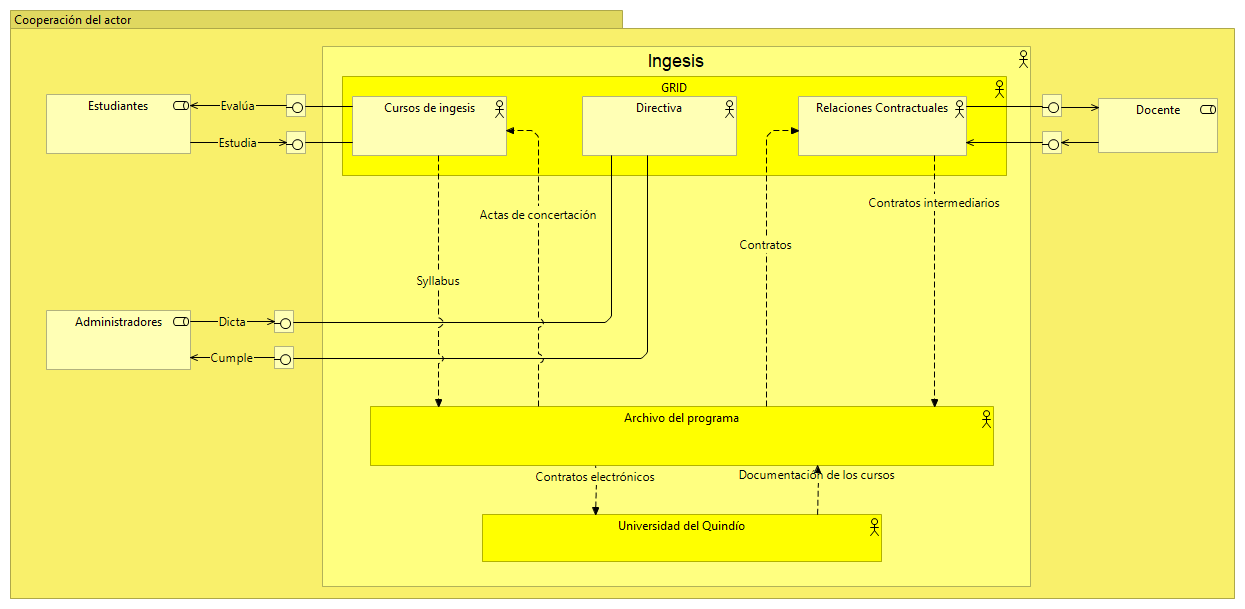
\includegraphics[width=0.9\textwidth]{mainmatter/II-desarrollo-metodologico/disenio/imagenes/cooperacion-actores.png}
	\caption{Vista de cooperación de actores}
	\label{fig:cooperacion-actores}
\end{figure}

\subsubsection{Vista de proceso de negocio}

La \autoref{fig:proceso-negocio} presenta la vista de proceso de negocio, cuyo propósito es modelar las actividades que conforman el ciclo de gestión de identidades y el proceso de autenticación de usuarios dentro de la solución propuesta. Esta vista permite comprender la secuencia lógica de las operaciones, los responsables involucrados y la información que interviene en cada etapa del proceso, independientemente de los componentes tecnológicos que posteriormente las implementan.

En el diagrama se identifican dos procesos principales. El primero corresponde a la gestión de usuarios, el cual inicia con la solicitud de creación o actualización de una cuenta por parte del administrador de tecnologías de la información. A continuación, se realiza la validación de la información suministrada, el procesamiento de los datos y la asignación de grupos y permisos, actividades que permiten generar o actualizar el registro del usuario y su pertenencia a los grupos correspondientes, de acuerdo con las políticas institucionales definidas. Como resultado del proceso se obtiene un usuario correctamente aprovisionado y preparado para acceder a los servicios institucionales.

El segundo proceso corresponde a la gestión de accesos, el cual inicia cuando un usuario solicita el inicio de sesión en alguno de los servicios integrados. Durante este proceso se validan las credenciales presentadas y posteriormente se verifican los permisos asociados a la cuenta, consultando los registros de usuarios, grupos y las políticas de acceso definidas. Si las validaciones son satisfactorias, el usuario obtiene acceso al servicio solicitado; en caso contrario, la autenticación o autorización es rechazada.

\begin{figure}[H]
	\centering
	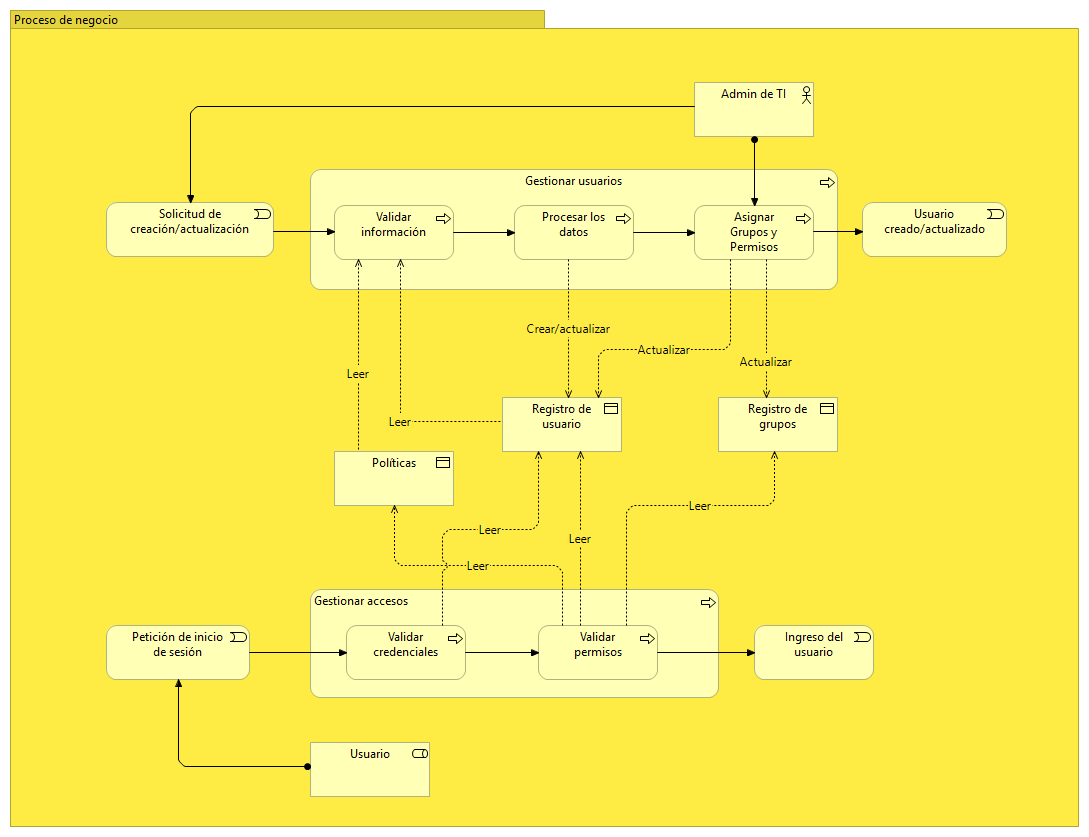
\includegraphics[width=0.9\textwidth]{mainmatter/II-desarrollo-metodologico/disenio/imagenes/proceso-negocio.png}
	\caption{Vista de procesos de negocio}
	\label{fig:proceso-negocio}
\end{figure}

\subsection{Vista de aplicación}

La \autoref{fig:servicios-aplicacion} presenta la vista de componentes y servicios de aplicación, cuyo propósito es describir la estructura lógica de la solución implementada y las interacciones entre los componentes que conforman el servicio de directorio centralizado. Esta vista permite identificar cómo cada componente de FreeIPA coopera para proporcionar los servicios de autenticación, autorización y gestión de identidades consumidos por las aplicaciones institucionales.

En el núcleo de la arquitectura se encuentra FreeIPA, representado como el contenedor lógico que integra los diferentes componentes responsables de la gestión de identidades. Entre estos se encuentra 389 Directory Server, encargado del almacenamiento y administración de la información del directorio \ac{LDAP}; Kerberos (\acs{KDC}), responsable de la autenticación mediante tickets y de la validación de identidades; Dogtag Certificate Authority, encargado de la emisión y administración de certificados digitales; Policy Engine, que implementa la evaluación de las políticas de autorización y control de acceso; y Web \acs{UI} + \ac{API}, que proporciona la interfaz administrativa y los servicios necesarios para la gestión del directorio.

El diagrama también muestra la cooperación entre estos componentes. El servicio de directorio constituye el repositorio central de identidades, siendo consultado por el servicio Kerberos durante los procesos de autenticación y por el motor de políticas para la evaluación de las reglas de autorización. De igual forma, la interfaz de administración consulta y actualiza la información almacenada en el directorio, mientras que la autoridad certificadora interactúa con esta para gestionar los certificados digitales asociados a usuarios y servicios.

\begin{figure}[H]
	\centering
	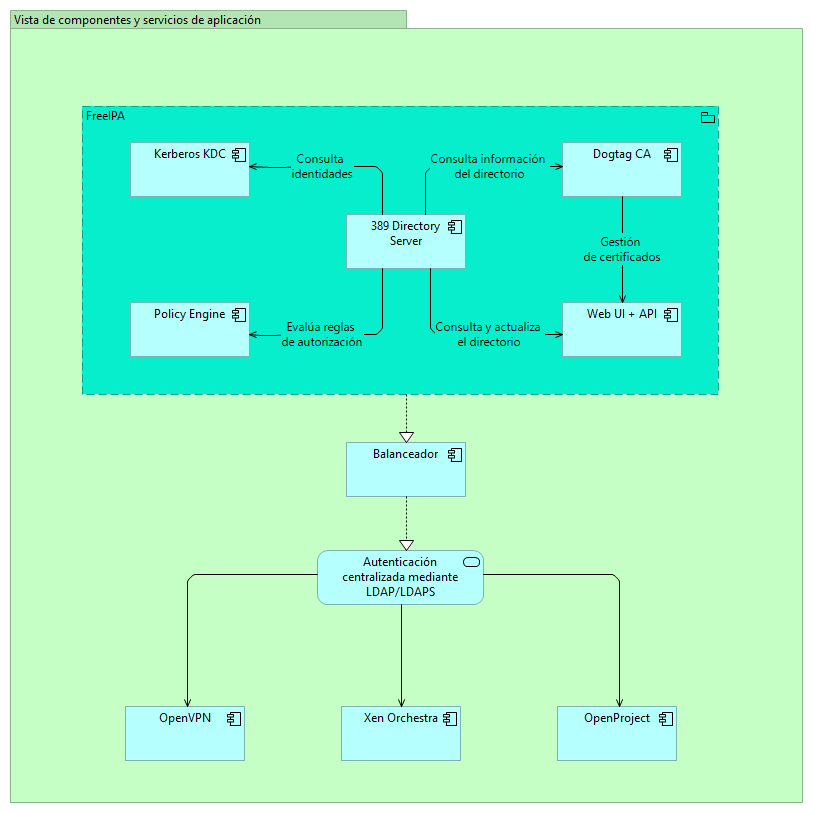
\includegraphics[width=0.9\textwidth]{mainmatter/II-desarrollo-metodologico/disenio/imagenes/servicios-aplicacion.png}
	\caption{Vista de componentes y servicios de aplicación de FreeIPA}
	\label{fig:servicios-aplicacion}
\end{figure}

\subsection{Capa de implementación}

La \autoref{fig:implementacion} presenta la vista de implementación, cuyo propósito es representar el despliegue físico y lógico de la solución dentro de la infraestructura tecnológica del Grupo de Investigación \ac{GRID}. Esta vista muestra la distribución de los servicios sobre el hipervisor, la organización de las máquinas virtuales, los mecanismos de comunicación entre ellas y los componentes que soportan la autenticación centralizada.

La arquitectura se encuentra desplegada sobre un hipervisor XCP-ng, el cual aloja las máquinas virtuales que conforman la solución. Estas se agrupan en dos dominios funcionales: el primero corresponde a los servidores de autenticación, donde se encuentran el servidor principal, el servidor réplica de FreeIPA y el balanceador de carga; el segundo agrupa las aplicaciones consumidoras, conformadas por OpenVPN, OpenProject y Xen Orchestra, cada una instalada sobre su respectivo sistema operativo y con los componentes adicionales requeridos para integrarse con el servicio de directorio.

En el servidor principal se despliegan los servicios que integran FreeIPA, incluyendo 389 Directory Server, Kerberos, Dogtag y el servicio \ac{LDAP}/\ac{LDAPS}, el cual constituye el punto de acceso utilizado por las aplicaciones para realizar procesos de autenticación y consulta de identidades. El servicio de directorio administra la información almacenada en la base de datos \ac{LMDB}, donde residen los datos del directorio \ac{LDAP} y sobre la cual se ejecutan las operaciones de creación, consulta, actualización y eliminación de registros. Paralelamente, el servidor réplica mantiene una copia sincronizada de estos componentes mediante un esquema de replicación Multi-Master \ac{LDAP}, garantizando la disponibilidad y continuidad del servicio ante fallos del nodo principal.

\begin{figure}[H]
	\centering
	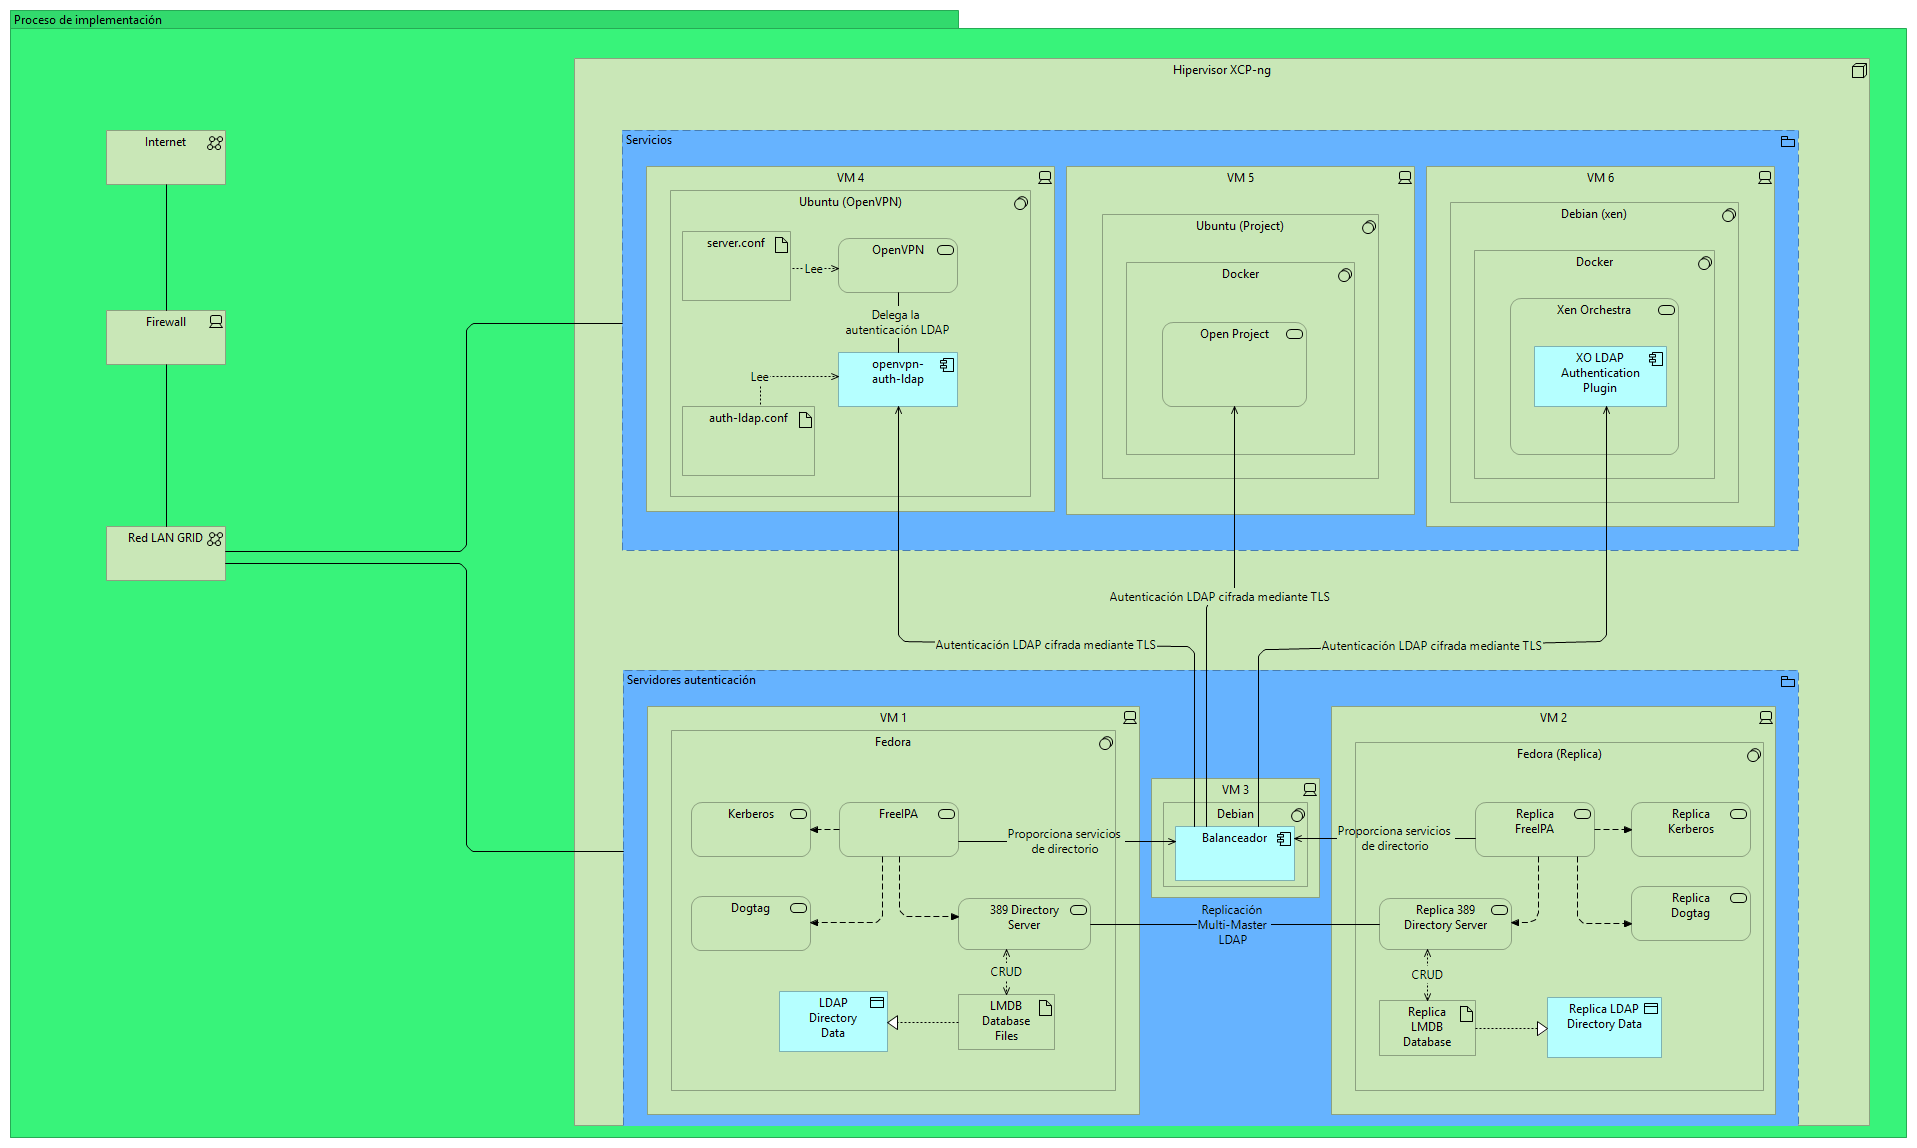
\includegraphics[width=0.9\textwidth]{mainmatter/II-desarrollo-metodologico/disenio/imagenes/implementacion.png}
	\caption{Vista de implementación de la arquitectura sobre la plataforma de virtualización}
	\label{fig:implementacion}
\end{figure}

\subsection{Capa de infraestructura}

La \autoref{fig:infraestructura} presenta la infraestructura física y de red sobre la cual se despliega la solución propuesta. En ella se observa la conectividad desde Internet hacia la red institucional de la Universidad del Quindío mediante un acceso seguro, así como la integración con la infraestructura del \ac{GRID}. El entorno de ejecución está soportado por un servidor físico que actúa como hipervisor, sobre el cual se alojan las máquinas virtuales que conforman la solución. Esta arquitectura proporciona una plataforma centralizada para el despliegue y administración de los servicios, garantizando la comunicación entre los diferentes componentes y ofreciendo una base escalable para futuras ampliaciones de la infraestructura.

\begin{figure}[H]
	\centering
	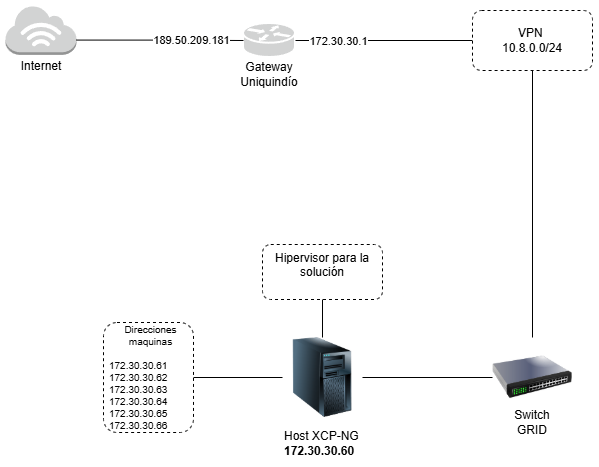
\includegraphics[width=0.9\textwidth]{mainmatter/II-desarrollo-metodologico/disenio/imagenes/infraestructura.png}
	\caption{Vista de infraestructura física y de red de la solución propuesta}
	\label{fig:infraestructura}
\end{figure}

\subsection{Capa de virtualización}

La \autoref{fig:virtualizacion} presenta la vista de virtualización, cuyo propósito es representar la distribución de las máquinas virtuales que conforman la solución dentro de la plataforma de virtualización utilizada. Esta vista permite identificar la organización de los recursos virtualizados, los sistemas operativos implementados y la ubicación lógica de cada uno de los servicios que integran la arquitectura.

La solución se encuentra desplegada sobre un hipervisor de tipo 1 XCP-ng, instalado directamente sobre el servidor físico, lo que proporciona un entorno de virtualización con acceso directo a los recursos de hardware, mejorando el rendimiento, la disponibilidad y el aislamiento entre las diferentes cargas de trabajo. Sobre esta plataforma se ejecutan seis máquinas virtuales, cada una destinada a un propósito específico dentro de la infraestructura.

Las dos primeras máquinas virtuales corresponden al servicio de directorio y están conformadas por un servidor principal FreeIPA y un servidor réplica FreeIPA, ambos implementados sobre el sistema operativo Fedora. Esta configuración permite disponer de redundancia en el servicio FreeIPA mediante la replicación y sincronización de la información del directorio entre ambos servidores, favoreciendo la continuidad del servicio de autenticación ante la indisponibilidad de uno de ellos. La sexta máquina virtual corresponde al balanceador de carga, cuya función es distribuir las solicitudes entre los servicios que requieren un único punto de acceso y que no cuentan con mecanismos propios de failover mediante servidores alternativos.

\begin{figure}[H]
	\centering
	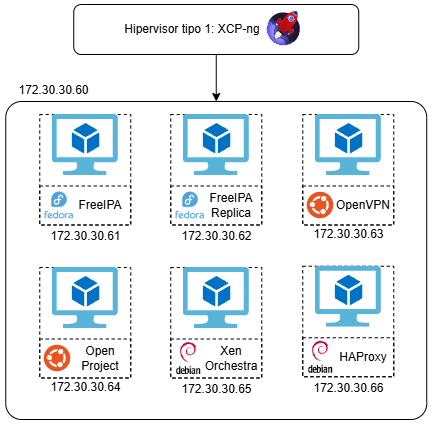
\includegraphics[width=0.9\textwidth]{mainmatter/II-desarrollo-metodologico/disenio/imagenes/virtualizacion.png}
	\caption{Vista de distribución de máquinas virtuales en el hipervisor XCP-ng}
	\label{fig:virtualizacion}
\end{figure}

\subsection{Vista por capas}

La \autoref{fig:capas} presenta la vista por capas de la arquitectura, cuyo propósito es proporcionar una visión integral de la solución propuesta, mostrando la relación existente entre las capas de negocio, aplicación e infraestructura. Esta vista permite comprender cómo los requerimientos funcionales de la organización son soportados por los componentes de software y cómo estos, a su vez, son desplegados sobre la infraestructura tecnológica.

En la capa de negocio se representan los actores involucrados en la administración y consumo del servicio de directorio, distinguiendo al Administrador de \ac{TI}, responsable de la gestión de identidades, y a los usuarios finales, representados por estudiantes y docentes, quienes consumen el servicio de autenticación centralizada. Asimismo, se identifican los servicios de negocio encargados de la administración de políticas, usuarios y grupos, además del servicio de autenticación y autorización que soporta el acceso a los recursos institucionales.

La capa de aplicación muestra la estructura lógica de FreeIPA y los componentes que cooperan para ofrecer los servicios de identidad. El 389 Directory Server actúa como repositorio central de usuarios, grupos y políticas; Kerberos proporciona los mecanismos de autenticación; Dogtag administra los certificados digitales; Policy Engine evalúa las reglas de autorización; y Web \acs{UI} + \ac{API} ofrece la interfaz para la administración del directorio. La interacción entre estos componentes permite implementar una plataforma unificada para la gestión de identidades y el control de acceso.

Finalmente, la capa de infraestructura representa el entorno sobre el cual se despliega la solución. En esta se observa un servidor físico que ejecuta un hipervisor encargado de alojar dos máquinas virtuales: una correspondiente al servidor principal de FreeIPA y otra destinada a la réplica del servicio. Ambas mantienen un mecanismo de replicación que permite mantener sincronizada la información del directorio y mejorar la disponibilidad del servicio ante la indisponibilidad de uno de los servidores.

Las relaciones entre las diferentes capas evidencian la trazabilidad de la arquitectura. Los servicios de negocio delegan la gestión de identidades y la autenticación en los componentes de FreeIPA, mientras que estos son soportados por la infraestructura de virtualización donde se encuentran desplegados el servidor principal y el servidor réplica. De esta manera, la vista permite relacionar los objetivos del negocio con los componentes tecnológicos que soportan la solución. La arquitectura resultante centraliza la gestión de identidades y establece mecanismos de control de acceso, replicación y balanceo orientados a proporcionar continuidad del servicio ante escenarios de indisponibilidad de uno de los servidores.

\begin{figure}[H]
	\centering
	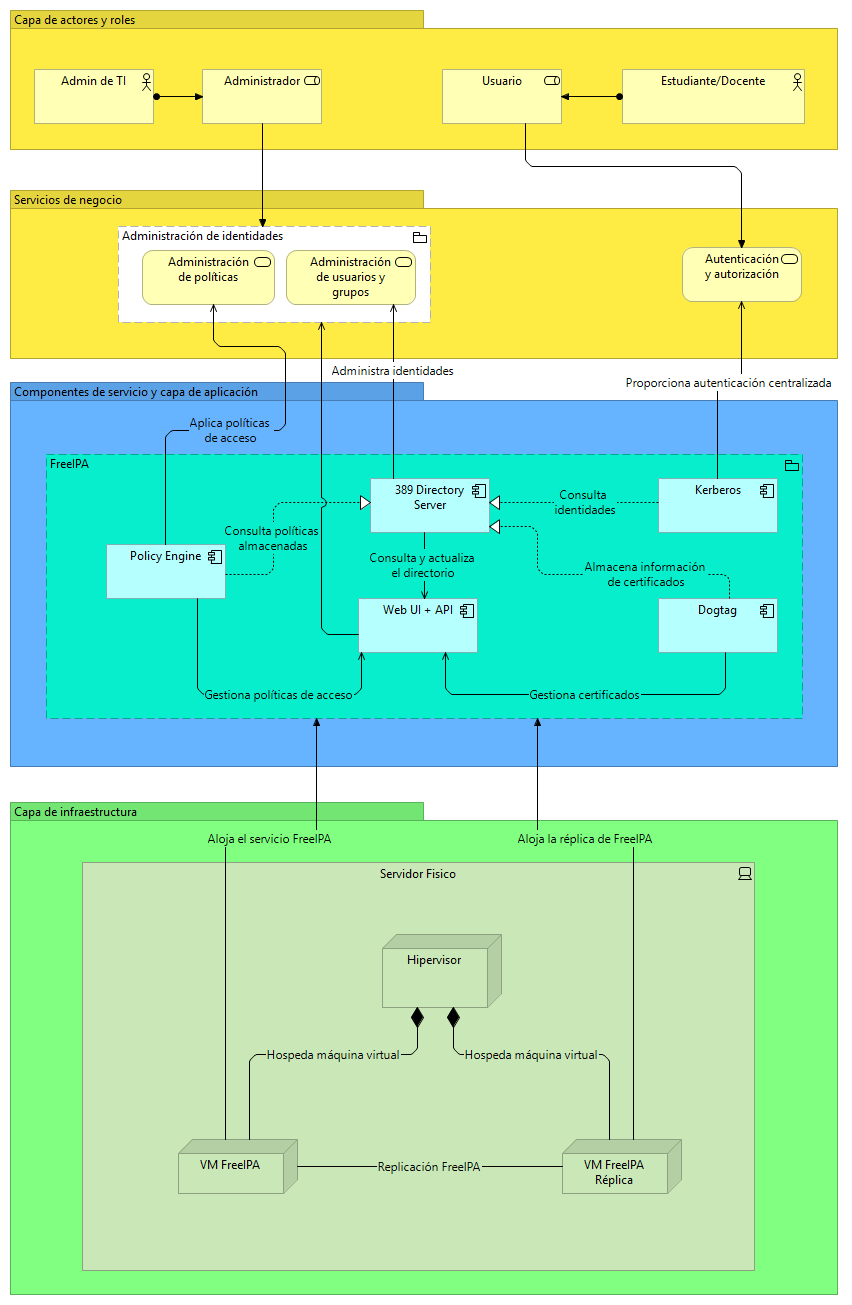
\includegraphics[width=0.9\textwidth]{mainmatter/II-desarrollo-metodologico/disenio/imagenes/capas.png}
	\caption{Vista por capas de la arquitectura}
	\label{fig:capas}
\end{figure}
